% HMC Math dept HW template example
% v0.04 by Eric J. Malm, 10 Mar 2005
\documentclass[10pt,a4paper,boxed]{hmcpset}

% set 1-inch margins in the document
% \usepackage[margin=1in]{geometry}
\usepackage{enumerate}
\usepackage{todonotes}
%\usepackage{tikz}
%\usetikzlibrary{positioning}
\usepackage{subfig} % subfigures in figures.	
\usepackage{pgfplots}
\usepackage{amsmath}
\usepackage{amsfonts}
\usepackage{amssymb}

%% work around for subfig and asy environment
\makeatletter
\newsavebox{\sfe@box}
\newenvironment{subfloatenv}[2]{%
\def\sfe@caption{#1}%
\def\sfe@label{#2}%
\setbox\sfe@box\hbox\bgroup\color@setgroup}%
{\color@endgroup\egroup\subfloat[\sfe@caption]%
{\usebox{\sfe@box}\label{\sfe@label}}}
\makeatother

% include this if you want to import graphics files with /includegraphics
\usepackage{graphicx}

\renewcommand*{\familydefault}{\sfdefault}
\newcommand{\vect}[1]{\mathbf{#1}}


%\tikzset{node distance=2cm, inner/.style={draw,circle}, leaf/.style={draw,rectangle}}

\usepackage{hyperref}

% info for header block in upper right hand corner
\name{Lukas Gesing, Patrick Kaster}
\class{MA-INF 4201 - Artificial Life}
\assignment{Exercise Sheet 4}
% \duedate{09/03/2004}

\begin{document}
\begin{problem}[Assignment 24]
\end{problem}
\begin{solution}
    A loop with the double length of the edges needs twice more \emph{msg.forward} blocks
    %\begin{figure}[h]
    %\centering
        %$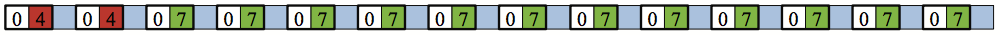
\includegraphics[width=1.0\textwidth]{LangtonsSelfReplicationLoopDouble.png}
    %\caption{Loop with the double length of the edges}
    %\end{figure}  
\end{solution}

\begin{problem}[Assignment 25]
\end{problem}
\begin{solution}
The reproduction of the \emph{Chou-Reggia}-loop is basically identical to \emph{Langton's loop}, except that in \emph{Chou-Reggia}-loop all sheaths are removed. Instead of the extending arm, a \emph{growth cap} is developed at the tip of the first \emph{msg.forward} blocks. This \emph{growth cap} provides a sense of orientation, replacing the function of the sheaths.

\begin{figure}[h!]
	\centering
	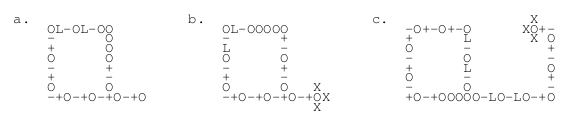
\includegraphics[width=0.8\textwidth]{img/choureggia}
	\caption{first three steps in replication of a \emph{Chou-Reggia}-loop. From \cite{ChouReggia}. }
\end{figure}
\end{solution}

%\begin{problem}[Assignment 26]
%\end{problem}
%\begin{solution}
%\end{solution}

\begin{problem}[Assignment 27]
\end{problem}
\begin{solution}
Let "$\vert$" be the concatenation of words. Then we have the following recursion for the L-system from the example:\\
\begin{align*}
	w_0 & = C, w_1 = A\\
	w_n & = w_{n-2} \vert w_{n-1} \\
	\vert w_n \vert & = \vert w_{n-2} \vert + \vert w_{n-1} \vert
\end{align*}
which is the recursion formula of the Fibonacci numbers ($\vert w_0 \vert = \vert w_1 \vert = 1$).

Proof of the recursion by induction:
	\begin{description}
		\item[Induction start: $n=2$;] $w_2 = w_0 \vert w_1 = C \vert A = CA$
		\item[Induction step: $n \rightarrow n+1$;] Using the induction hypothesis we conclude: $w_{n+1} = w_{(n+1)-2} \vert w_{(n+1)-1} = w_{n-1} \vert w_n$
	\end{description}
\end{solution}

\begin{problem}[Assignment 28]
\end{problem}
\begin{solution}
	\begin{tabular}{ll}
	 variables: & R, S, T\\ 
	 axiom: & R \\
	 		& \\
	 rule 1: & $R \rightarrow RS$ \\
	 rule 2: & $S \rightarrow ST$ \\
	 rule 3: & $T \rightarrow TR$ \\
	\end{tabular}
\end{solution}

\newpage

\begin{problem}[Assignment 29]
\end{problem}
\begin{solution}
	\begin{enumerate}[a)]
		\item 
			The $B \rightarrow B C$ rule adds one unit length per turn, thus controls the length of the segments. The $A \rightarrow A +B C +B C$ concatenates the turns of the spiral
			%\begin{table}[h!]
				\begin{tabular}{ll}
					 variables: & A, B, C\\ 
					 constants: & +,- \\
					 axiom: & -A \\
							& \\
					 rule 1: & $A \rightarrow A +B C +B C$ \\
					 rule 2: & $B \rightarrow B C$ \\
				\end{tabular}
			%\end{table}

		\item 
			%\begin{table}[h!]
				\begin{tabular}{ll}
					 variables: & B, C, D, E, F\\ 
					 constants: & +,- \\
					 axiom: & B \\
						    & \\
					 rule 1: & $B \rightarrow C [-B] E [+B]$ \\
					 rule 2: & $C \rightarrow F[-D]F$ \\
					 rule 3: & $F \rightarrow FF$
				\end{tabular}
			%\end{table}
	\end{enumerate}
	\begin{figure}[h]
		\centering
		\begin{subfloatenv}{spiral for $\alpha=12^\circ$, $100$ iterations}{fig:spiral}
			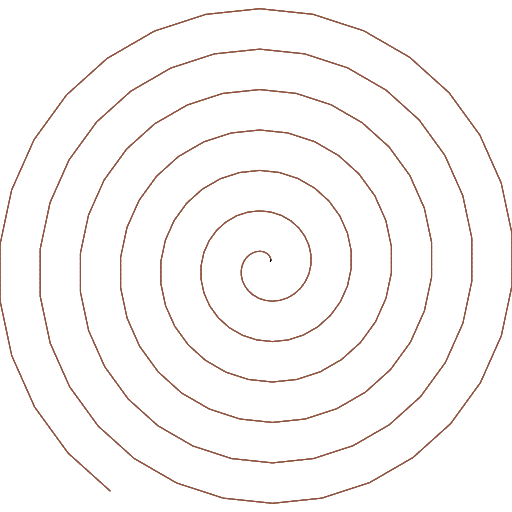
\includegraphics[width=0.3\textwidth]{img/spiral}
		\end{subfloatenv}
		\begin{subfloatenv}{tree, for $\alpha=30^\circ$, $5$ iterations}{fig:tree}
			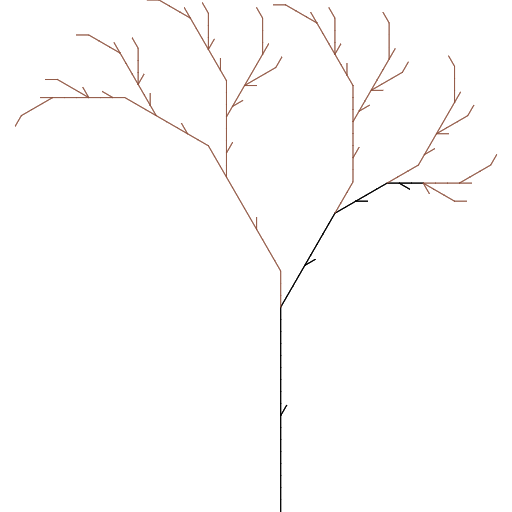
\includegraphics[width=0.3\textwidth]{img/tree}
		\end{subfloatenv}
		%\caption{proof by induction over points on a circle}
			% das label muss immer nach der caption kommen, sonst gibt es Probleme bei der Referenzierung und Nummerierung.
		\label{fig:plots}
	\end{figure}
\end{solution}

\pagebreak

%\begin{problem}[Assignment 30]
%\end{problem}
%\begin{solution}
%\end{solution}

\begin{thebibliography}{[01]}
\bibitem[01]{ChouReggia} Reggia, James A and Chou, Hui-Hsien and Lohn, Jason D: "Cellular automata models of self-replicating systems" published in "Advances in Computers", volume 47, pp. 141--183, \emph{Elsevier}, 1998

\end{thebibliography}

\end{document}
